\chapter{Introduction}

Elementary particle physics aims to describe nature at its most fundamental level.
This thesis presents analyses of data obtained from high energy proton collisions, which search for evidence for or against new theoretical models of elementary particle physics.
This section introduces the theoretical context of these searches, describing first the theoretical model presently serving as the null hypothesis of elementary particle physics, then a few issues identified with this model, and finally some proposed solutions for these issues.

\section{The Standard Model of Particle Physics} \label{sec:standardmodel}

Modern elementary particle physics finds itself in a peculiar state.
Physicists have constructed a theoretical model, now called the Standard Model of Particle Physics (the Standard Model; SM), that is the most quantitatively accurate scientific model of any kind, consistent with experiment in almost every laboratory test, even when experimental uncertainty is smaller than a part per ten billion \cite{electronmu_exp,electronmu_th}, with its most famously accuract prediction displayed in Table~\ref{tab:electronmu}.
\begin{table}
\centering
\begin{tabular}{r l}
\multicolumn{2}{c}{$\mu_e$} \\
\hline
Experiment & 2.00231930436 (56) \\
Theory & 2.002319304363 (15)
\end{tabular}
\caption[Comparison of theoretical prediction and experimental measurement of the electron magnetic moment.]
        {A comparison of the leading experimental measurement of the electron's magnetic moment \cite{electronmu_exp}, and the Standard Model's theoretical prediction \cite{electronmu_th}, in terms of the classical prediction, the Bohr magneton. 
          Famously, this is the most accurate verification of theory by experiment in all of science. 
          The numbers in parentheses are the uncertainties, on the same order as the last digits printed.}
\label{tab:electronmu}
\end{table}

It is important to take this time to reflect on the Standard Model's astonishing accuracy, because the Standard Model is known with certainty to be imperfect, for a few reasons. 
A subset are discussed in Section~\ref{sec:SMproblems}.
Particle physicists have a theory {\it known} to be incomplete, only an approximation, and yet so accurate an approximation that no evidence in favor of any specific proposed extension has ever been found.
Modern particle physicists hope to find experimental clues by testing the Standard Model using any available means, including by comparing its predictions for the outcomes of high energy proton collisions with experimental data.

  \subsection{A Brief Description} \label{sec:SMdescription}

  The Standard Model is based in quantum field theory (QFT), which provides the general toolkit used to make calculations, and identifies the observed elementary particles as excitations of these underlying fields.
  Since every elementary particle corresponds directly to an underlying field and vice-versa, for example ``the electron particle'' and ``the electron field'' are colloquially treated as synonyms.

  The SM itself, like every model of elementary particle physics based in QFT, consists of a list of particles present in nature and a description of their interactions with each other.
  The particles can be grouped in several ways, but by far the most significant is to group bosons and fermions.

  The bosons of the Standard Model are the photon (typically indicated by $\gamma$), the W$^+$ and W$^-$, the Z, the eight gluons, and the Higgs.
  Of these, the Higgs has no intrinsic angular momentum (``spin-0'') and the others have intrinsic angular momentum of exactly $\hbar$ (``spin-1'').
  One of the major insights obtained from QFT is that the existence of spin-1 particles requires the existence of fermions that interact with them, and vice versa.
  A fermion that interacts with a boson is said to be ``charged under'' the boson.
  Moreover, pure fermion interactions are forbidden, so that fermion-fermion interactions require a ``mediating'' boson under which both fermions are charged, while boson-boson interactions are perfectly acceptable.
  For this reason, bosons are said to mediate fundamental interactions.
  The photon mediates electromagnetism, and the gluons collectively mediate the strong interaction, as described by quantum chromodynamics (QCD).
  For historical reasons, the distinct interactions mediated by the W$^+$ and W$^-$, the Z, and the Higgs are all collectively called the weak interaction.
  The bosons of the Standard Model are summarized in Table~\ref{tab:bosons}.

  \begin{table}
    \centering
    \begin{tabular}{r r l}
      Boson             & Mass (GeV) \cite{pdg} & Interaction \\
      \hline
      Photon ($\gamma$) & 0                     & Electromagnetism \\
      Gluon (g)         & 0                     & Strong (QCD) \\
      W$^{\pm}$         & 80.379 $\pm$ 0.012    & Weak (charged current) \\
      Z                 & 91.1876 $\pm$ 0.0021  & Weak (neutral current) \\
      Higgs (h)         & 125.18 $\pm$ 0.16     & Weak (symmetry breaking and mass) \\
    \end{tabular}
    \caption[Table of Standard Model bosons.]
            {The Standard Model bosons, their masses, and associated interactions. Note that there are eight gluons, but they are not experimentally distinct.}
            \label{tab:bosons}
  \end{table}

  The interactions have very different character due to differences in the mediating bosons.
  The photon and electromagnetism are most familiar.
  Electromagnetism is relatively simple, as a result of having only a single-component charge and a single mediating boson, and is relatively easily studied due to its long range, as a consequence of the masslessness of the photon.
  The weak interaction, by contrast, is less well-known in part due to its very short range, a consequence of the {\it large} masses of the mediating bosons.
  In addition to the $1/r^2$ behavior familiar from electromagnetism, forces are also suppressed by an exponential term, $e^{-\frac{mc^2}{\hbar c}r}$, where $m$ is the mass of the mediating boson and $\hbar c \approx 200$~GeV-pm.
  This term vanishes for massless bosons like the photon, but since the weak bosons have masses on the order of 100~GeV, the weak interaction becomes negligible after only a few picometers despite having an intrinsic interaction strength comparable to electromagnetism.
  Thus, the weak interaction has an impact only on nuclear and elementary particle physics.
  The strong interaction is also short ranged, with effects becoming significant only on the order of femtometers, but for an entirely different reason.
  As its name suggests, it is also intrinsically stronger than the other interactions.
  It will be discussed in Section~\ref{sec:hadronization}.

  The fermions of the Standard Model are all spin-$\frac{1}{2}$, and come in two major groups.
  The leptons are those fermions which do not participate in the strong interaction, and the quarks are those that do.
  The leptons can be further subdivided into the electrically charged leptons, like the electron, and the electrically neutral neutrinos, which having neither strong nor electromagnetic interactions can interact only weakly, and are ghostlike particles as a result.
  The quarks can be further subdivided into the up-type quarks, which are positively charged, and the down-type quarks, which are negatively charged.
  There are three of each quark, one for each of the charges of the strong interaction, but like the eight gluons, they are not experimentally distinct.

  As is evident in Table~\ref{tab:fermions}, the fermions of the Standard Model occur in triplets with identical properties aside from mass: the up-type quarks, the down-type quarks, the charged leptons, and the neutrinos are all roughly three versions of the same particle with different masses.
  The fermions are therefore said to be arranged in three similar generations, with generation 1 having the least mass and generation 3 the greatest.

  \renewcommand{\arraystretch}{1.2}
  \begin{table}
    \centering
    \begin{tabular}{l c r r}
      Fermion             & Symbol & Mass (GeV) \cite{pdg} & Electric charge \\
      \hline
      Up quark            & $u$    & $0.0022^{+0.0005}_{-0.0004}$      & +$\frac{2}{3}$  \\
      Charm quark         & $c$    & $1.275^{+0.025}_{-0.035}$       & +$\frac{2}{3}$  \\
      Top quark           & $t$    & $173.0 \pm 0.4$       & +$\frac{2}{3}$  \\
      Down quark$^*$      & $d$    & $0.0047^{+0.0005}_{-0.0003}$      & -$\frac{1}{3}$  \\
      Strange quark       & $s$    & $0.095^{+0.009}_{-0.003}$       & -$\frac{1}{3}$  \\
      Bottom quark        & $b$    & $4.18^{+0.04}_{-0.03}$       & -$\frac{1}{3}$  \\
      \hline
      Electron            & $e$    & $0.0005109989461$(31) & $-1$ \\
      Muon                & $\mu$    & $0.1056583745$(24)  & $-1$ \\
      Tau                 & $\tau$    & $1.77686$(12)  & $-1$ \\
      Neutrinos           & $\nu_{e}$, $\nu_{\mu}$, $\nu_{\tau}$ & 0$^{\dagger}$ & 0 \\
    \end{tabular}
    \caption[Table of Standard Model fermions.]
    {A table of the Standard Model fermions, first the quarks then the leptons.
      The vastly different experimental character of quarks due to their confinement by the strong interactions make their masses much more difficult to measure than those of the charged leptons.
      Note that every Standard Model fermion also has an antiparticle, with identical properties except for opposite charge.
      (*) The charge and mass eigenstates of (by convention) down-type quarks are different, so that for example ``the mass of the down quark'' does not exist. Otherwise, decays across generations would be impossible. In practice, they are so nearly equal that the mass of the down quark is equated with that of the lightest mass eigenstate, etc.
      ($\dagger$) The Standard Model predicts that neutrinos are massless but they experimentally have nonzero masses, albeit one million times smaller than the electron's (see Section~\ref{sec:SMproblems}).
}
            \label{tab:fermions}
  \end{table}
  \renewcommand{\arraystretch}{1}

  If each generation were truly independent of the others, then each would be independently stable, as there would be no way to cross from, say, generation 3 to generation 1.
  However, it is an experimental fact that quarks can decay across generations via their interactions with the W boson, albeit much more slowly than within generations.
  This is well-accomodated in the Standard Model \cite{cabibbo,ckm}, in which there is no reason in general for the charge eigenstates with respect to any given boson to be equal to those of any other.
  Famously, the Higgs boson is responsible for the masses of the Standard Model's elementary particles, with each particle acquiring a mass proportional to the strength of its interaction with the Higgs.
  The Higgs interaction eigenstates, being the mass eigenstates, are priviliged as the only charge eigenstates that are also eigenstates of the Hamiltonian, and so are the only states that can actually be produced.
  The hybrid nature of the physical states with respect to W interactions produces effective generation-crossing interactions for quarks described by the Cabibbo-Kobayashi-Maskawa (CKM) matrix, with values measured experimentally to be approximately \cite{pdg},
  \begin{equation} \label{eqn:ckm}
    \begin{bmatrix} 
      |V_{ud}| & |V_{us}| & |V_{ub}| \\
      |V_{cd}| & |V_{cs}| & |V_{cb}| \\
      |V_{td}| & |V_{ts}| & |V_{tb}| 
    \end{bmatrix}
\approx
    \begin{bmatrix} 
      0.974 & 0.224 & 0.004 \\
      0.218 & 0.997 & 0.042 \\
      0.008 & 0.039 & 1.019
    \end{bmatrix}
  \end{equation}
  where $V_{xy}$ indicates the effective coupling between quarks $x$ and $y$.
  If the eigenstates were exactly equal, the CKM matrix would be diagonal, with $V_{xx} = 1$ and $V_{xy} = 0$ ($x \neq y$), prohibiting trans-generation decays.
  As can be seen in Equation~\ref{eqn:ckm}, the CKM matrix is {\it nearly} diagonal, meaning trans-generation decays are slow but not impossible.
  This causes the bottom quark to have a longer lifetime than the charm quark despite having a larger mass, because a bottom quark must cross a generation to decay  (the top quark is more massive) using $|V_{ub}| \approx 0.004$ or $|V_{cb}| \approx 0.042$, while a charm quark does not (the strange quark is less massive) and may decay using $|V_{cs}| \approx 0.997$.
  In fact, the bottom quark lifetime is long enough that bottom hadron decay lengths are macroscopic, on the order of millimeters.
  This is experimentally relevant, as discussed in Section~\ref{sec:btagging}.
  Similar physics is possible for leptons since neutrinos are now known to be massive, but is not incorporated in the Standard Model, in which neutrinos are massless (see Section~\ref{sec:SMproblems}).

  The detailed interactions of the Standard Model are more conveniently discussed using Feynman Diagrams, in the next section.

  \subsection{Feynman Diagrams and Perturbative Expansions} \label{sec:feyndiags}

  The interactions of the Standard Model are expressed as a Langrangian density, of intimidating complexity.
  Applying the Euler-Lagrange equations to this Lagrangian produces nonlinear differential equations that have no known exact solutions.
  However, it is possible to extract an approximate solution as a perturbative expansion in powers of the coupling, a parameter that indicates the intrinsic strength of an interaction.
  This procedure at first seems barely feasible, as it is no trivial task to find all the contributions to the leading order term, then the next to leading order term, and so on by simple inspection of the Lagrangian.
  Fortunately, physicist Richard Feynman was able to devise a diagrammatic method for expressing the terms of the perturbative expansion that is far more intuitive.

  First, one may inspect each term of the Lagrangian to assemble so-called vertices, the building blocks of diagrams.
  Each field that occurs in a term represents one line, and all the lines of a term intersect at a central point to form the vertex.
  For example, the Standard Model Lagrangian contains a term in which the electron field appears twice and the photon field appears once, from which one obtains the vertex shown in Figure~\ref{fig:eegamma}.
  Each vertex represents one power of the coupling.
  The diagrams with the fewest vertices, then, are the lowest order diagrams in the perturbative expansion.

  \begin{figure}[h!]
    \centering
    \begin{fmffile}{eegamma}
      \begin{fmfgraph*}(40,25)
        \fmfleft{i1,i2}
        \fmfright{o1,o2}
        \fmfbottom{b}
        \fmf{fermion,label=$e^-$,label.side=left}{i2,v1}
        \fmf{fermion,label=$e^-$,label.side=left}{v1,o2}
        \fmf{photon,label=$\gamma$,label.side=left}{v1,b}
      \end{fmfgraph*}
    \end{fmffile}

    \caption[The fundamental vertex of electromagnetism.]{
      The Standard Model Lagrangian contains a term in which the electron field appears twice, and the photon field once, which corresponds to this Feynman diagram vertex.
      This vertex, and analogous vertices in which another electrically charged fermion replaces the electron, are the vertices of electromagnetism.      
      Traditionally, straight lines with arrows represent fermions, and a wavy line represents a photon (or a W or Z).
      The arrows on fermion lines mark whether a fermion is matter or antimatter, depending on whether the arrow points generally in the same (matter) or opposite (antimatter) direction as the flow of time (left to right).
    }
    \label{fig:eegamma}
  \end{figure}  

  Typically, time runs left to right in Feynman diagrams.
  The vertex in Figure~\ref{fig:eegamma}, then, depicts an incoming electron absorbing or emitting a photon, and continuing along.
  All Feynman vertices can be freely rotated, effectively changing the flow of time.
  For example, one can rotate Figure~\ref{fig:eegamma} to produce Figure~\ref{fig:eeannihilation}.
  Figure~\ref{fig:eeannihilation} depicts the annihilation of an electron and its antiparticle, the positron, into a photon.
  While this process is allowed by the Standard Model as shown, it is not allowed kinematically, as it is impossible to conserve energy and momentum with only a single massless particle in the final state.
  To produce the leading order diagram for electron-positron annihilation that is allowed by kinematics, two vertices must be {\it connected} as shown in Figure~\ref{fig:eeannihilation_allowed}, by attaching two identical external lines.

  \begin{figure}[h!]
    \centering
    \begin{fmffile}{eeannihilation}
      \begin{fmfgraph*}(40,25)
        \fmfleft{i1,i2}
        \fmfright{o1}
        \fmf{fermion,label=$e^-$,label.side=left}{i2,v1}
        \fmf{fermion,label=$e^+$,label.side=left}{v1,i1}
        \fmf{photon,label=$\gamma$,label.side=left}{v1,o1}
      \end{fmfgraph*}
    \end{fmffile}

    \caption[A rotation of the fundamental vertex of electromagnetism.]{
      This diagram is a rotation of Figure~\ref{fig:eegamma}.
      Instead of an incoming electron absorbing or emitting a photon, this diagram represents an electron and its antiparticle, the positron, annihilating into a photon.
      While permitted as an interaction by the Standard Model, this process is not kinematically allowed, making Figure~\ref{fig:eeannihilation_allowed} the leading order diagram for electron-positron annihilation.
    }
    \label{fig:eeannihilation}
  \end{figure}  

  \begin{figure}[h!]
    \centering
    \begin{fmffile}{eeannihilation_allowed}
      \begin{fmfgraph*}(40,25)
        \fmfleft{i1,i2}
        \fmfright{o1,o2}
        \fmf{fermion,label=$e^-$,label.side=left}{i2,v2}
        \fmf{fermion,label=$e$,label.side=left}{v2,v1}
        \fmf{fermion,label=$e^+$,label.side=left}{v1,i1}
        \fmf{photon,label=$\gamma$,label.side=left}{v1,o1}
        \fmf{photon,label=$\gamma$,label.side=left}{v2,o2}
      \end{fmfgraph*}
    \end{fmffile}

    \caption[The leading order diagram of electron-positron annihilation.]{
      This diagram connects vertices like those of Figures~\ref{fig:eegamma}~and~\ref{fig:eeannihilation} to produce the leading order kinematically allowed diagram for electron and positron annihilation.
      Whether the internal line is an electron or positron is ambiguous, due to the relativity of simultaneity.
      In some reference frames, the positron emits a photon first, then annihilates with the electron, and so the internal line is a positron.
      In others, the electron emits a photon first, then annihilates with the positron, and the internal line is an electron.
    }
    \label{fig:eeannihilation_allowed}
  \end{figure}  

  All of the diagrams shown thus far have been ``tree-level,'' with no internal loops.
  These tend to be the leading order diagrams, but diagrams with internal loops also contribute to the amplitude, usually at sub-leading order.
  Figure~\ref{fig:eeannihilation_loop} is one such diagram, contributing to the next-to-leading order term of the electron-positron annihilation amplitude.

  \begin{figure}[h!]
    \centering
    \begin{fmffile}{eeannihilation_loop}
      \begin{fmfgraph*}(40,25)
        \fmfleft{i1,i2}
        \fmfright{o1,o2}
        \fmf{fermion}{i2,vi}
        \fmf{fermion}{vi,v2}
        \fmf{photon,right=1}{vi,vf}
        \fmf{fermion}{v2,vf}
        \fmf{fermion}{vf,v1}
        \fmf{fermion}{v1,i1}
        \fmf{photon}{v1,o1}
        \fmf{photon}{v2,o2}
      \end{fmfgraph*}
    \end{fmffile}

    \caption[One of the next-to-leading order diagrams of electron-positron annihilation, containing an internal loop.]{
      This diagram is one of the next-to-leading order contributions to the electron-positron annihilation amplitude, containing an internal loop.
    }
    \label{fig:eeannihilation_loop}
  \end{figure}  

  In all of the diagrams we have reviewed thus far, the electron could be replaced with any electrically charged fermion, such as a muon or up quark.
  Collectively, all of these diagrams and others like them, constructed by combining variants of Figure~\ref{fig:eegamma}, constitute electromagnetism.

  The strong interaction as described by Quantum Chromodynamics (QCD) has a similar foundational diagram, shown in Figure~\ref{fig:qcdvertices} (upper), in which the photon is switched out for a gluon, and the fermion must be a quark.
  Unlike electromagnetism, the strong interaction also contains interactions between the mediating bosons, the gluons, alone.
  These vertices are partly responsible for the dramatically different physics of the strong interaction compared to electromagnetism.
  See Section~\ref{sec:hadronization} for more details.

  \begin{figure}[h!]
    \centering
    \begin{fmffile}{qqgluon}
      \begin{fmfgraph*}(40,25)
        \fmfleft{i1,i2}
        \fmfright{o1,o2}
        \fmfbottom{b}
        \fmf{fermion,label=$q$,label.side=left}{i2,v1}
        \fmf{fermion,label=$q$,label.side=left}{v1,o2}
        \fmf{gluon,label=$g$,label.side=left}{v1,b}
      \end{fmfgraph*}
    \end{fmffile}

    \begin{fmffile}{g3}
      \begin{fmfgraph*}(40,25)
        \fmfleft{i1,i2}
        \fmfright{o1,o2}
        \fmfbottom{b}
        \fmf{gluon,label=$g$,label.side=left}{i2,v1}
        \fmf{gluon,label=$g$,label.side=left}{v1,o2}
        \fmf{gluon,label=$g$,label.side=left}{v1,b}
      \end{fmfgraph*}
    \end{fmffile}

    \begin{fmffile}{g4}
      \begin{fmfgraph*}(40,25)
        \fmfleft{i1,i2}
        \fmfright{o1,o2}
        \fmf{gluon,label=$g$,label.side=left}{i1,v1}
        \fmf{gluon,label=$g$,label.side=left}{i2,v1}
        \fmf{gluon,label=$g$,label.side=left}{v1,o1}
        \fmf{gluon,label=$g$,label.side=left}{v1,o2}
      \end{fmfgraph*}
    \end{fmffile}

    \caption[The vertices of QCD.]{
      The Standard Model Lagrangian contains terms in which appear (upper) one of the quark fields twice, and a gluon field once, (middle) 3 separate gluon fields, and (lower) 4 gluon fields.
      These are the vertices of QCD.      
      Unlike the lines of other bosons, gluon lines are traditionally drawn as springs.
    }
    \label{fig:qcdvertices}
  \end{figure}  

  Finally, some of the vertices of the weak interaction are shown in Figure~\ref{fig:weakvertices}.

  \begin{figure}[h!]
    \centering
    \begin{fmffile}{qqW}
      \begin{fmfgraph*}(40,25)
        \fmfleft{i1,i2}
        \fmfright{o1,o2}
        \fmfbottom{b}
        \fmf{fermion,label=$q_u$,label.side=left}{i2,v1}
        \fmf{fermion,label=$q_d$,label.side=left}{v1,o2}
        \fmf{photon,label=$W$,label.side=left}{v1,b}
      \end{fmfgraph*}
    \end{fmffile}

~

    \begin{fmffile}{lnuW}
      \begin{fmfgraph*}(40,25)
        \fmfleft{i1,i2}
        \fmfright{o1,o2}
        \fmfbottom{b}
        \fmf{fermion,label=$\ell$,label.side=left}{i2,v1}
        \fmf{fermion,label=$\nu_{\ell}$,label.side=left}{v1,o2}
        \fmf{photon,label=$W$,label.side=left}{v1,b}
      \end{fmfgraph*}
    \end{fmffile}

~

    \begin{fmffile}{ffZ}
      \begin{fmfgraph*}(40,25)
        \fmfleft{i1,i2}
        \fmfright{o1,o2}
        \fmfbottom{b}
        \fmf{fermion,label=$f$,label.side=left}{i2,v1}
        \fmf{fermion,label=$f$,label.side=left}{v1,o2}
        \fmf{photon,label=$Z$,label.side=left}{v1,b}
      \end{fmfgraph*}
    \end{fmffile}

~

    \begin{fmffile}{ffH}
      \begin{fmfgraph*}(40,25)
        \fmfleft{i1,i2}
        \fmfright{o1,o2}
        \fmfbottom{b}
        \fmf{fermion,label=$f$,label.side=left}{i2,v1}
        \fmf{fermion,label=$f$,label.side=left}{v1,o2}
        \fmf{dashes,label=$h$,label.side=left}{v1,b}
      \end{fmfgraph*}
    \end{fmffile}

    \caption[The vertices of QCD.]{
      The Standard Model Lagrangian contains terms in which appear (upper) an up-type quark field and down-type quark field once each, and the W field once, (second) a similar diagram with a charged lepton and its associated neutrino replacing the quarks, (third) a fermion field appears twice, and the Z field once, and (lower) a non-neutrino fermion field appears twice, and the Higgs once.
      These are the vertices of the weak interaction that include both fermions and bosons.      
      The weak interaction also includes many boson-only interactions similar to Figure~\ref{fig:qcdvertices} (lower), but these are omitted for brevity.
      The Z diagram (third) is very similar to the interaction of the photon with fermions, with the important addition that the fermion here can also be an electrically-neutral neutrino.
      The lines of spin-0 bosons are traditionally drawn as dotted lines, as in the lower diagram.
    }
    \label{fig:weakvertices}
  \end{figure}  

  In order to calculate rates and distributions of elementary particle physics processes, one assembles diagrams using the minimal number of vertices, then the next to minimal number, and so forth up to the desired precision, then follows an algorithm to convert each diagram to its equivalent mathematical expression.
  The result of evaluating this expression is the quantum mechanical amplitude for the process.
  This tedious procedure is now performed almost entirely by computers, using software such as the MadGraph generator \cite{madgraph}.

  \subsection{Quantum Chromodynamics, Hadronization, and Jets} \label{sec:hadronization}

  Quantum Chromodynamics is the theory of the strong interactions incorporated into the Standard Model, describing the interactions of quarks and gluons.
  States that are neutral with respect to the strong interactions (``colorless,'' to avoid confusion with electromagnetic neutrality) that are composed of quarks are called hadrons, analogous to atoms of electromagnetism.
  There are two distinct ways to create a colorless state, due to the unique 3-component structure of the QCD charge.
  The first is to have a quark and antiquark with +1 and -1 units, respectively, of the same component of the QCD charge.
  These cancel each other out in fashion similar to a proton and electron in electromagnetism, forming a hadron called a meson.
  The second is to have 3 quarks, each with 1 unit of a different component of the QCD charge, or 3 antiquarks each with -1 unit of a different component.
  This kind of hadron is called a baryon, and there is no electromagnetic analogue to this kind of neutral object.
  The only stable hadron is the proton, the lightest baryon, excepting neutrons bound to protons by the QCD equivalent of dipole forces in atomic nuclei.
  The formation of hadrons is called hadronization, and the hadronization process after a high energy collision tends to produce objects called jets that are important in experiments.
  
  To understand hadronization and jets, it is necessary to understand a feature of the strong interaction intimately related to why it is short ranged despite having a massless mediator, as was mentioned in the previous sections.
  Unlike the familiar electromagnetism, in which the potential energy associated with two charges decreases as the separation of the changes increases, the QCD potential energy increases without bound as two quarks are separated, roughly linearly proportional to distance \cite{lattice_potential}, as shown in Figure~\ref{fig:QCDpotential}.
  Eventually, the potential energy stored in the quark system exceeds the rest energy of a new hadron, and it becomes energetically preferable to convert some of the energy stored in the gluon fields into new hadrons, creating a new quark-antiquark pair and resetting the separation distance, than to allow further separation of the quarks.
  As a result, any attempt to separate two quarks cannot ultimately succeed, and all quarks are bound inside colorless hadrons. 
  As gluons {\it also} carry color charge (that is, gluons interact with themselves as shown in Figure~\ref{fig:qcdvertices}), they are similarly confined, and the reach of the strong interaction is limited to only a few femtometers.

  \begin{figure}[h!]
    \centering
    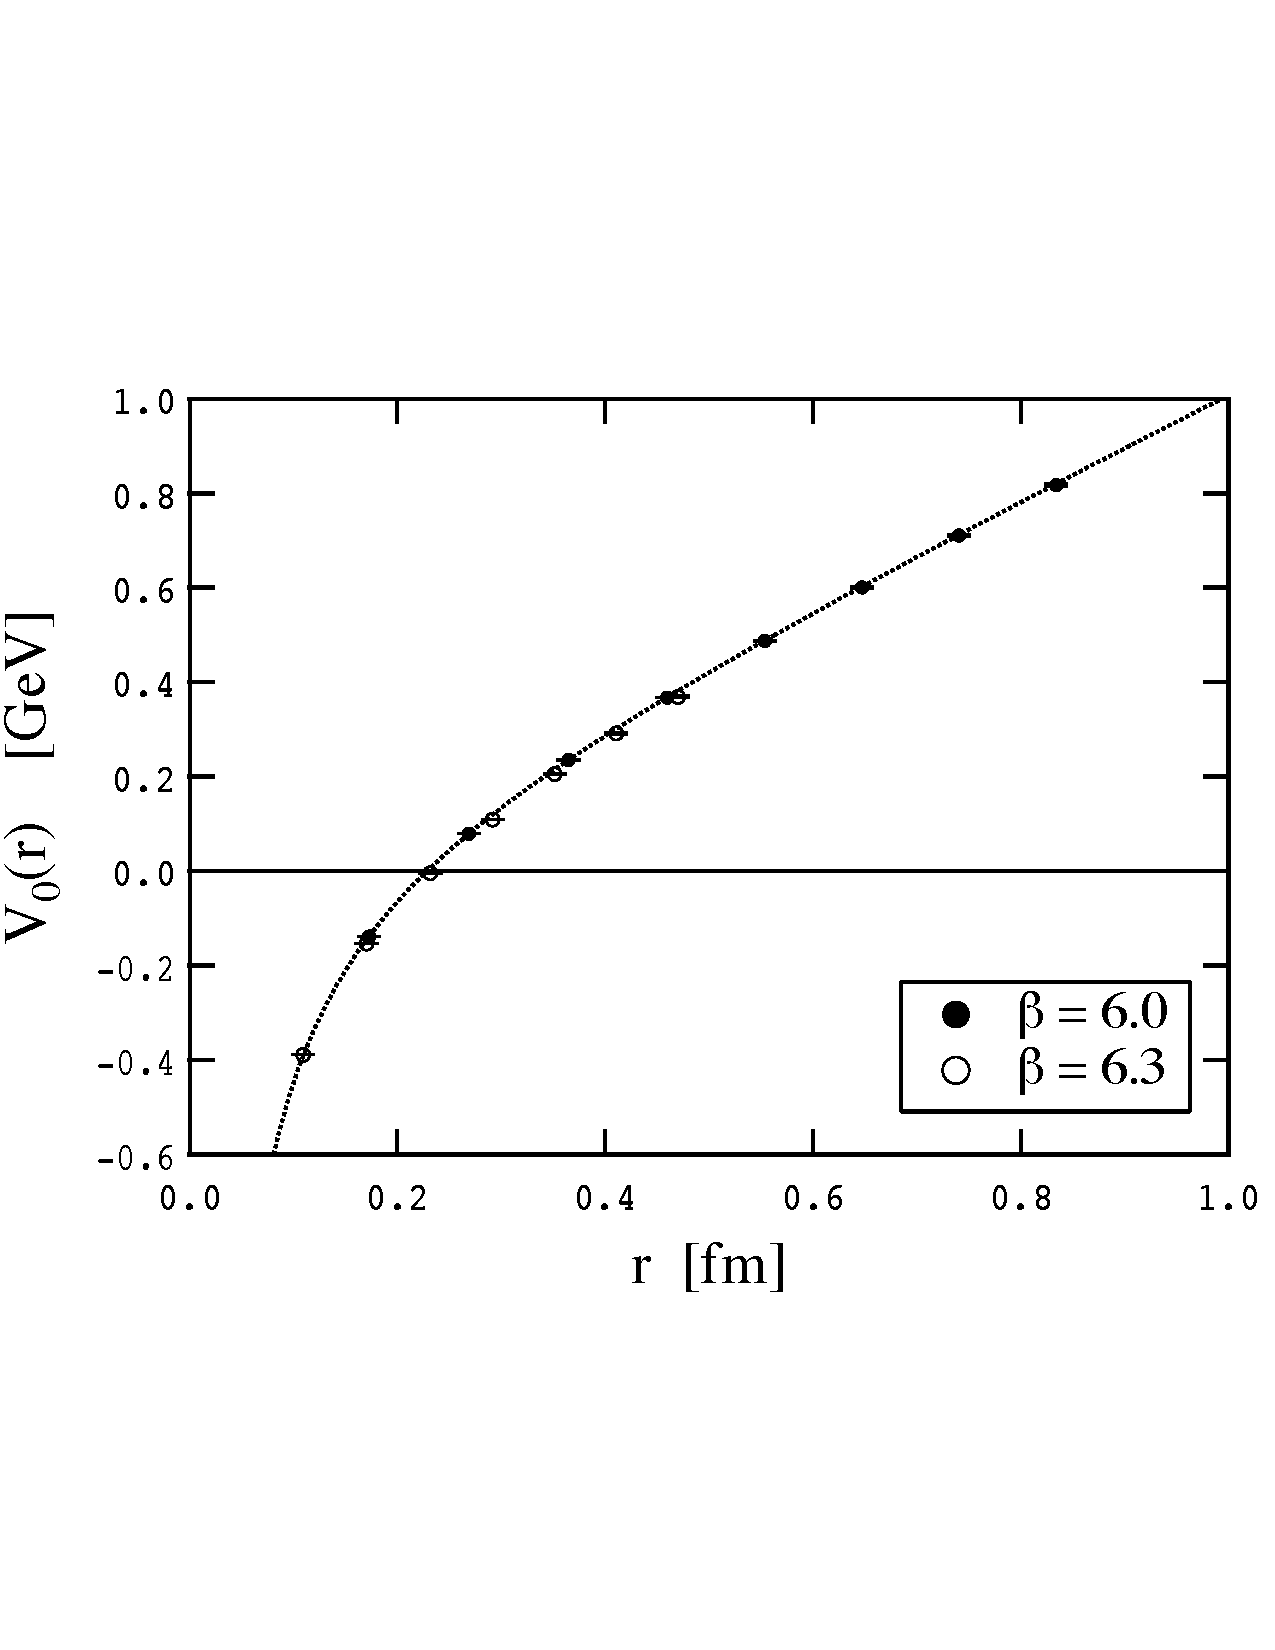
\includegraphics[width=0.4\textwidth]{figures/lattice_potential_qcd.pdf}
    \caption[Tracker material budget.]{
      The potential energy associated with two static quarks predicted by QCD as a function of distance, calculated numerically using the lattice technique.
      The potential increases roughly linearly with distance once a quark is no longer inside a hadron.
      The strong coupling used for the numerical calculation is denoted by $\beta$.
      Taken from \cite{lattice_potential}.}
    \label{fig:QCDpotential}
  \end{figure}  

  During a high energy collision involving a hadron like a proton, quarks and gluons are customarily ejected, and eventually reach a great enough distance to trigger the formation of new hadrons.
  But, the ejection is oftentimes so violent that even this new hadron fragments into new daughter hadrons, then these fragment, and so on.
  This fragmentation process produces a spray of hadrons, hadron decay products, and hadrons formed from QCD radiation analogous to bremstrahhlung, all traveling in approximately the same direction as the original ejected quark or gluon, which are collectively called a hadron jet.

  Unfortunately, while the production of jets is understood qualitatively, it is difficult to predict quantitatively due to yet another peculiar feature of QCD.
  The perturbative expansion described in the previous section is performed in powers of the interaction's coupling, with one factor of the coupling per vertex.
  In order for a truncated perturbation series to be a good approximation, the coupling must be significantly less than 1.
  Otherwise, diagrams with more vertices are in general more important than diagrams with fewer vertices, and no finite truncation can be accurate.
  Although the QCD coupling is less than 1 at high energy, making the perturbative approach still viable for very high energy collisions, the coupling explodes at low energies, which earns the strong interaction its name.

  \begin{figure}[h!]
    \centering
    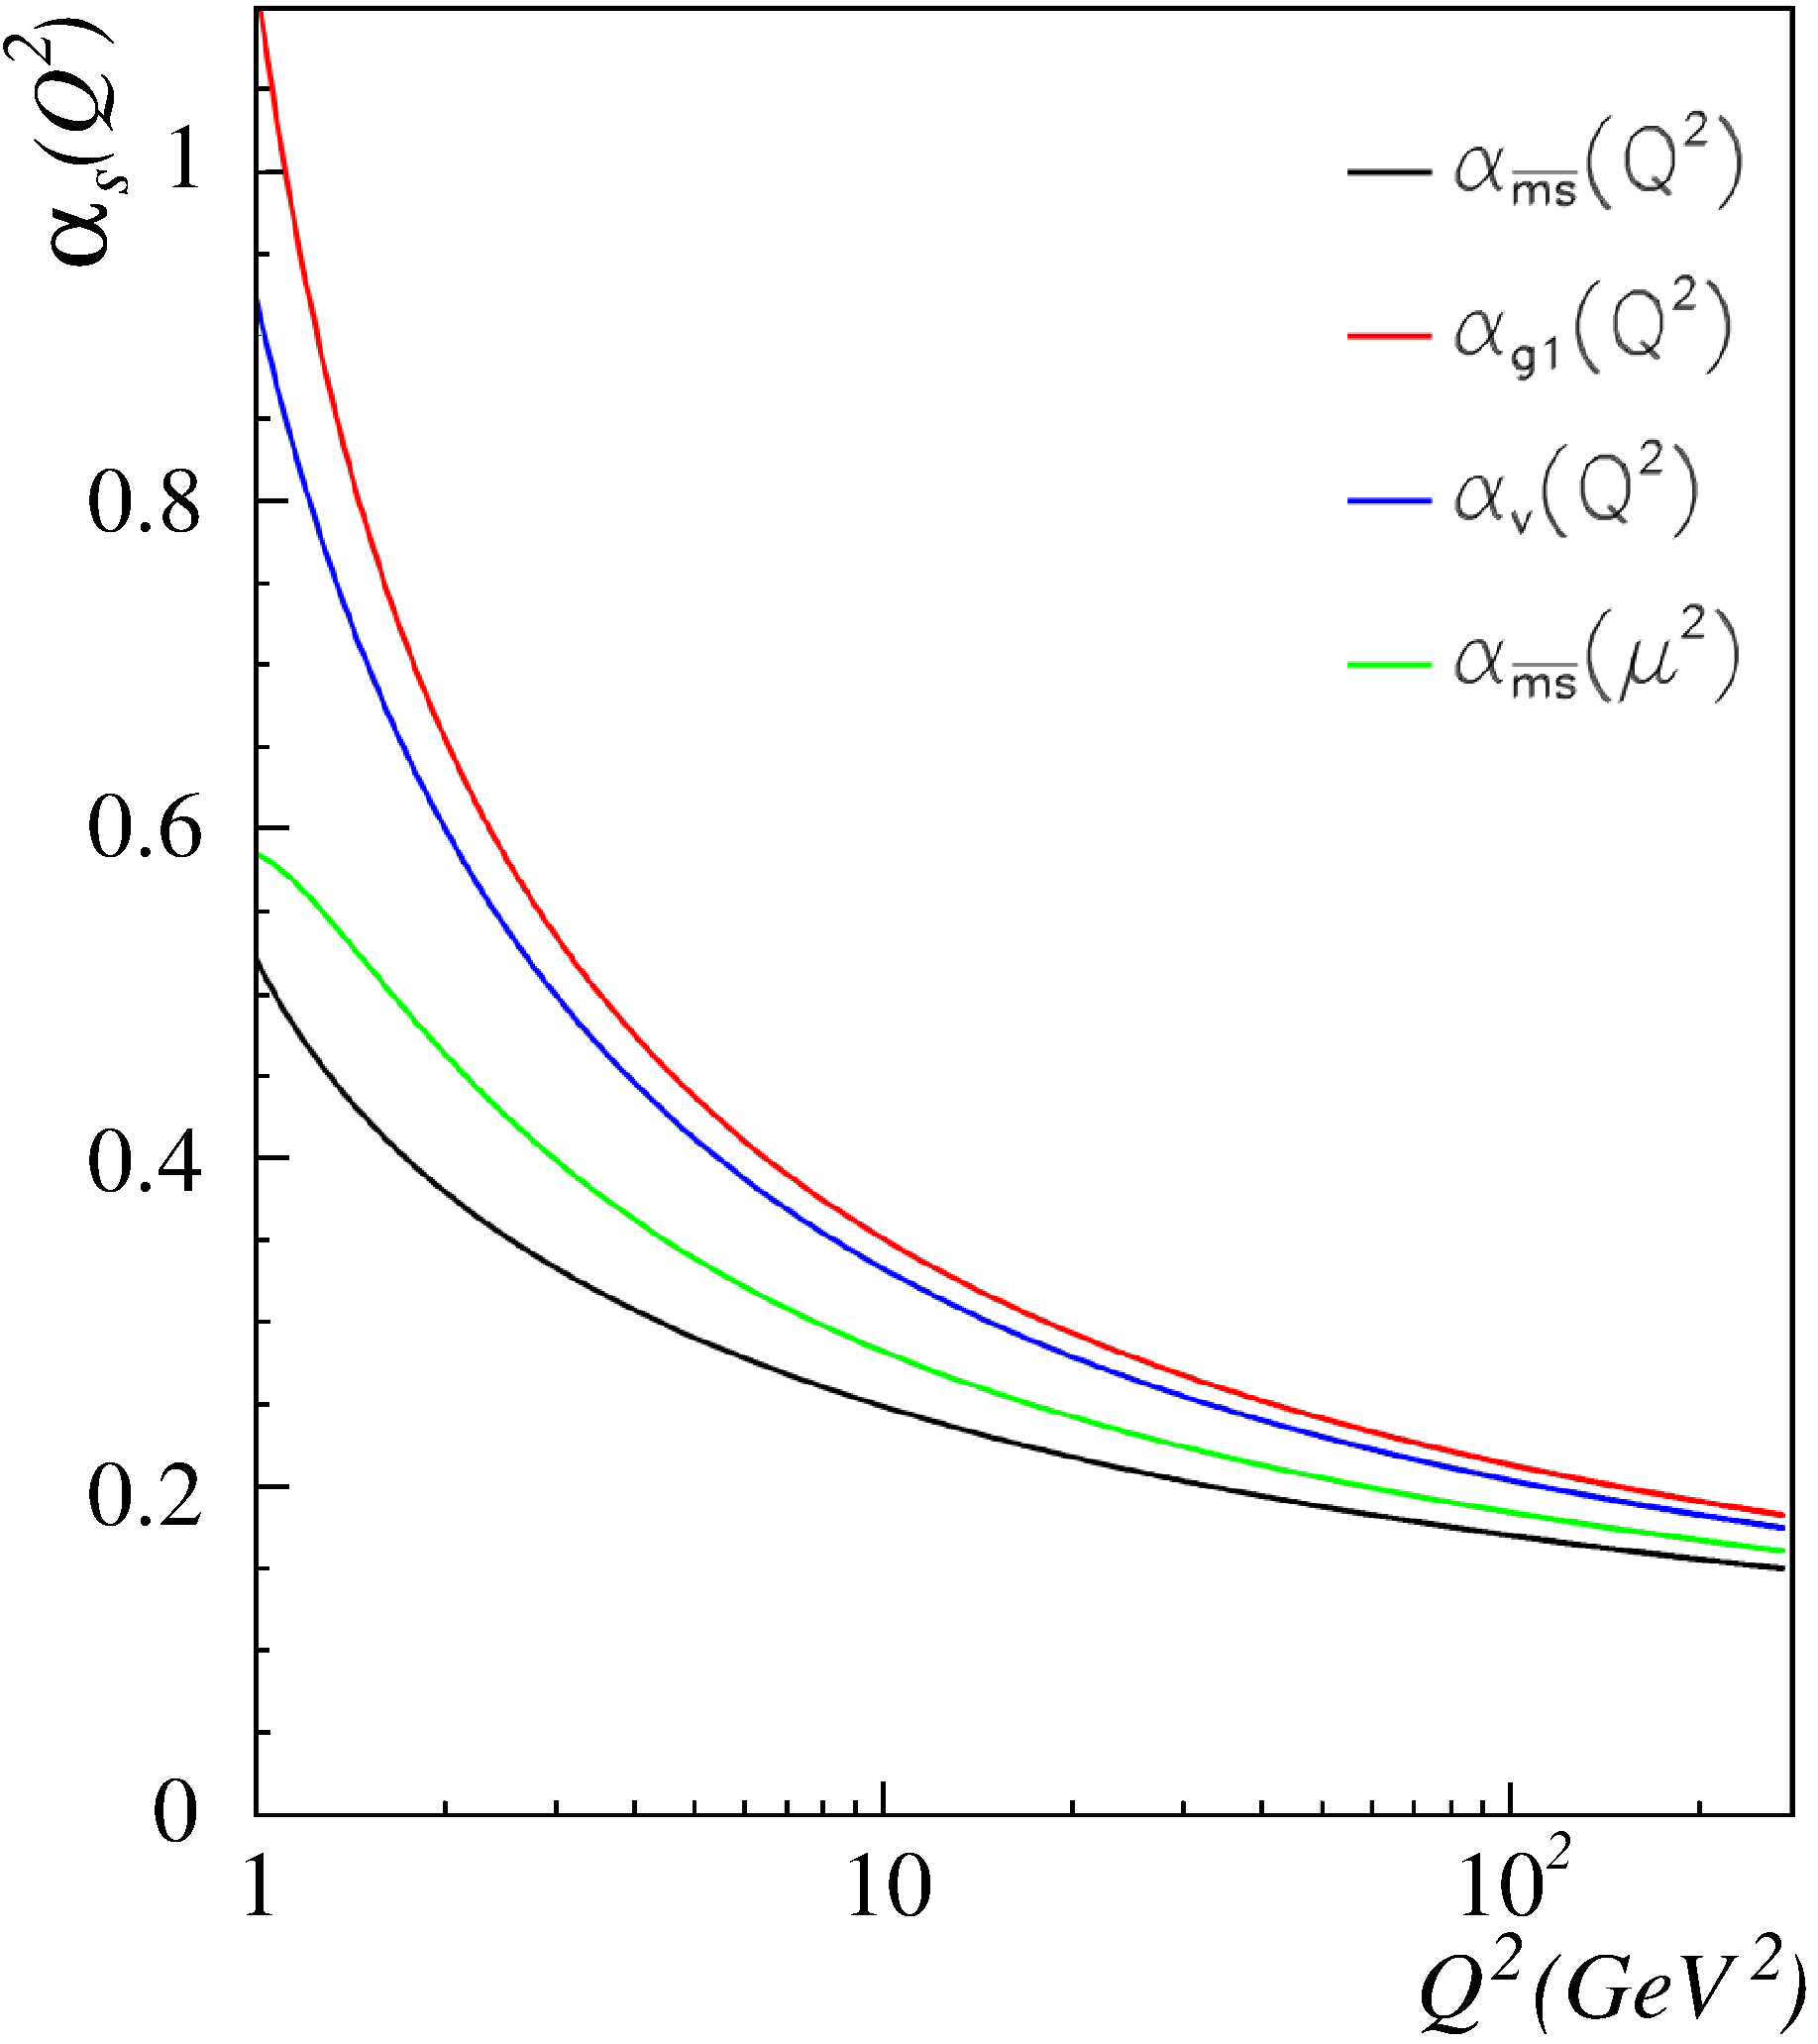
\includegraphics[width=0.4\textwidth]{figures/qcd_coupling.pdf}
    \caption[The QCD coupling as a function of the interaction energy.]{
      The QCD coupling explodes at low energy, making QCD non-perturbative for any interaction energy below around 1~GeV.
      The different lines are obtained for different methods of performing the calculation, specifically different renormalization schemes.
      Taken from \cite{qcd_coupling}.}
    \label{fig:QCDcoupling}
  \end{figure}  

  Non-perturbative approaches to QCD exist, including the lattice numerical method used to produce the plot shown in Figure~\ref{fig:QCDpotential}, but they are extremely computationally expensive for even the most simple calculations.
  It is not feasible to use make non-perturbative calculations of low energy QCD physics from first principles in an environment as complex as high energy hadron collisions.
  For the hadronization and fragmentation process, heuristic approximations tweaked to match data are used instead, typically the Lund String Model as implemented in the Pythia software package (see Section~\ref{sec:simulation}).
  Additionally, relatively low energy quarks and gluons can be emitted during the collision itself, called Initial State Radiation (ISR).
  A diagram of $u\bar{u} \rightarrow Z \rightarrow e^+e^-$ that includes a single ISR gluon is shown in Figure~\ref{fig:ISRdiag}.
  The most reliable way to predict ISR is to measure it in a very similar physics process, then convert this measurement to an expected rate in the physics process of interest.
  For example, ISR in $Z\rightarrow e^+e^-$ events is essentially identical to ISR in $Z\rightarrow \nu\nu$ events.
  
  \unitlength=2mm
  \begin{figure}[h!]
    \centering
    \begin{fmffile}{ISRdiag}
      \begin{fmfgraph*}(40,25)
        \fmfleft{i1,i2}
        \fmfright{o1,o2}
        \fmfbottom{b}
        \fmf{fermion,label=$u$,label.side=left}{i2,v1}
        \fmf{fermion,label=$\bar{u}$,label.side=left}{i1,vi}
        \fmf{fermion}{vi,v1}
        \fmf{gluon,label=ISR gluon,label.side=left}{vi,b}
        \fmf{photon,label=$Z$,label.side=left}{v1,v2}
        \fmf{fermion,label=$e^-$,label.side=left}{o2,v2}
        \fmf{fermion,label=$e^+$,label.side=left}{v2,o1}
      \end{fmfgraph*}
    \end{fmffile}

    \caption[A Feynamn diagram including an ISR gluon.]{
      Relatively low energy QCD can lead to the emission of Initial State Radiation as part of the hard collision, in this case $u\bar{u} \rightarrow Z \rightarrow e^+e^-$.
      This gluon will hadronize and add a jet to the event.
      ISR is difficult to predict accurately due to the intractability of QCD at low energy.
    }
    \label{fig:ISRdiag}
  \end{figure}  

  In summary, QCD's intractability at low energy combined with its raw strength make precise predictions of the outcome of hadron collisions difficult to obtain, despite the Standard Model's overall success in describing the interactions of elementary particles.
  The Standard Model prediction cannot always be obtained directly from first principles with satisfactory accuracy.

  \subsection{Parton Distribution Functions} \label{sec:PDFs}

  Being composite particles bound by QCD, the internal structure of hadrons is rich and difficult to understand quantitatively, due to the impossibility of using perturbation theory at the low energies that prevail in hadrons.
  Of greatest interest is the internal structure of the proton, the only stable hadron.
  The proton is often said to be a bound state of two up quarks and one down quark.
  This is true enough---the {\it net} composition of a proton is two up quarks and one down quark---but is an oversimplification.
  The quarks in a proton constantly emit and absorb gluons, which can split to quark-antiquark pairs, which can in turn annihilate back to gluons.
  Viewed at a small enough length scale, the proton is not a simple object, and not even a bound state of 3 quarks, but rather a complex cloud of quarks and gluons with various energies.
  This is problematic for any attempt to predict the outcome of proton collisions, because one cannot be sure which of these subcomponents, called partons, will be the component of the proton that actually experiences a collision.
  Due to the intractability of QCD at low energy, the composition of a proton is known only from a fit to data, and called a Parton Distribution Function (PDF).
  PDFs are typically expressed as the probability to find a parton of a given species carrying a given fraction of the proton's energy, as shown in Figure~\ref{fig:PDF}.
  These PDFs display a few sensible features described in the figure's caption.
  A large number of proton collisions collectively sample all the possible initial partons, with momentum distributions described by the PDFs.
  Thus, a dataset composed of proton collisions naturally probes a wide range of collision energies with a variety of colliding particles, making proton collisions well-suited to searches for new particles of unknown properties.

  \begin{figure}[h!]
    \centering
    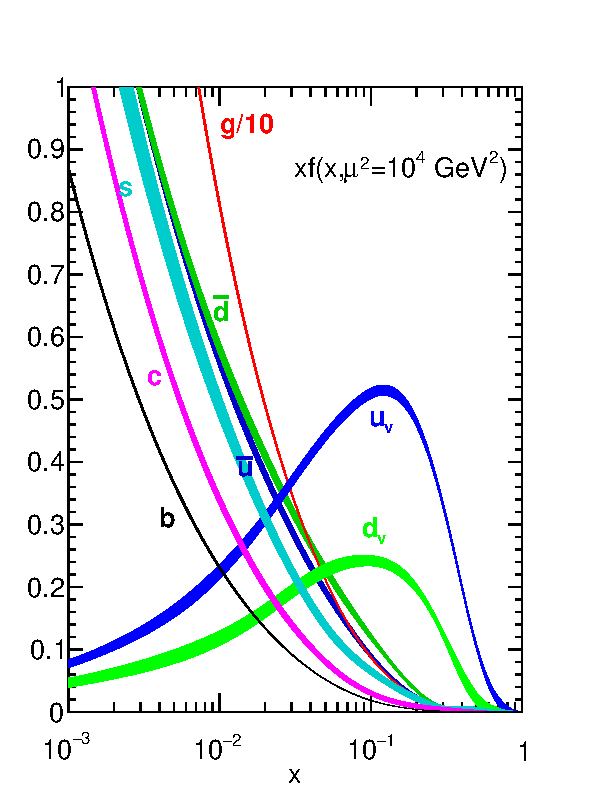
\includegraphics[width=0.4\textwidth]{figures/parton_distribution_function.pdf}
    \caption[Proton parton distribution function.]{
      The measured parton distribution function for a proton at an interaction energy of 100~GeV.
      The horizontal axis $x$ is the fraction of the proton's total momentum, and the vertical axis is the probability distribution.
      The finite thickness of the curves indicates the uncertainty.
      As one would expect for a proton, $uud$, the probability to collide with an up quark is around twice the probability to collide with a down quark at any energy.
      The $v$ subscript on these two curves indicate that these are the ``valence'' quarks, the only quarks that are present as more than transient products of gluon splitting.
      It is much less likely to find an up or down antiquark, and roughly equally likely to find either, because these antiquarks are produced only by gluons splitting to quark-antiquark pairs.
      Since they are also produced only transiently by gluon splitting, the probability to find a heavier quark, namely $s$, $c$, or $b$, is exactly equal to the probability to find a heavy antiquark.
      Quarks aside, notice that the gluon curve (red) has been suppressed by a factor of 10 to fit on the plot.
      To a decent approximation, high energy proton colliders in practice collide gluons.
      Taken from \cite{PDFs}.}
    \label{fig:PDF}
  \end{figure}  


\section{Some Problems with the Standard Model} \label{sec:SMproblems}

The Standard Model is extremely successful, as epitomized by the result in Table~\ref{tab:electronmu}, but not entirely satisfactory.
In fact, its success in laboratory experiments is a source of frustration for elementary particle physicists, as there are precious few hints as to how its deficiencies can be repaired.
This section introduces a few of the known problems with the Standard Model.

  \subsection{Gravity, and the Standard Model as an Effective Field Theory} \label{sec:gravity}

  In Section~\ref{sec:standardmodel}, there is never any mention of gravity as an interaction between particles.
  This is because the Standard Model entirely omits gravity from its description of nature, which means the Standard Model cannot possibly be the final theory.
  Instead, the Standard Model must be only an {\it effective theory}, a model of nature that applies only below some cutoff energy at which it is replaced by a more fundamental theory.
  In the case of the Standard Model, this cutoff cannot be any larger than the energy at which gravity becomes relevant in the interactions of elementary particles.

  Unlike the fields of the Standard Model, whose couplings are dimensionless, the gravitational coupling $G$ has dimensions of inverse energy squared.
  An old effective field theory of the weak interactions developed by Enrico Fermi, which modeled the weak interactions of fermions without mediating bosons, had a similar coupling, $G_F \approx \frac{1}{(100\mathrm{~GeV})^2}$.
  The energy scale embedded in the couling was a message from the theory, hinting that the theory would need to be replaced by something more fundamental in order to model physics at the scale of around 100~GeV or more.
  Nowadays, we recognize this energy as the mass scale of the weak interaction's mediating bosons.
  At interaction energies on the order of 100~GeV or larger, there is enough energy to produce the boson itself as a resonant excitation of the field, a real particle, and the underlying theory is revealed.
  Making an analogous inference from the gravitational coupling, one obtains the maximum possible cutoff energy for the Standard Model, the so-called Planck Energy of around $10^{19}$~GeV, at which gravity must be incorporated into the quantum theory.

  Moreover, the Standard Model becomes self-inconsistent at very high energies, even ignoring the gravity problem \cite{landaupole,higgstriviality}.
  The couplings of both electromagnetism and of the Higgs to itself increase with increasing energy, until eventually diverging at very high energy scales, a theoretical consistency issue called quantum triviality.
  As a result, the Standard Model's formulation of electromagnetism cannot be used for any energy greater than around $10^{34}$~GeV \cite{laundaupole}.
  Although this energy is far greater than the Planck energy, at which the Standard Model must fail anyway due to its exclusion of gravity, it is a completely independent indication that the Standard Model must be only a low energy limit of some more fundamental theory that supersedes it at high energy, and does not exhibit these kinds of problems.
  Even if one supposes that gravity's exclusion from the Standard Model is not actually a problem, that attempting to treat gravity like the other interactions is misguided, the Standard Model still cannot be the final theory.
  The Higgs self-interaction similarly diverges above the Planck scale, although had the Higgs mass turned out to be only around 200~GeV rather than the measured 125~GeV, the problem would arise below the Planck scale, and a Higgs mass as small as around 600~GeV would have made the triviality scale only a few TeV, accessible to current experiments \cite{higgstriviality}.

  Thus, there exist known finite energy scales at which the Standard Model {\it must} fail, both due to its exclusion of gravity and internal mathematical consistency issues, and the actual cutoff energy may be much smaller than these upper limits.
  Every experiment probing an unexplored energy scale has a chance to be the first to observe a hint as to what this more fundamental theory looks like.

  \subsection{The Hierarchy Problem} \label{sec:hierarchy}

  As described in the previous section, the energy scales of the weak interaction and of gravity differ by approximately 17 orders of magnitude.
  If the Standard Model emerges from some more fundamental theory at the Planck energy, then what effect has pushed the weak scale down 17 orders of magnitude?
  The most troublesome expression of this apparently inexplicable hierarchy of energy scales centers on the mass of the Higgs boson.
  In the Standard Model, the Higgs mass $m_h$ is given approximately by \cite{SUSYnaturalness,higgsmass},
  \begin{equation} \label{eqn:higgsmass}
    m_h^2 \approx 2\mu^2 + (\Delta m_h)^2
  \end{equation}
  where $\mu$ is the so-called bare mass of the Higgs, and $\Delta m_h$ is an adjustment that the Higgs acquires via its interactions with other fields in the Standard Model,
  \begin{equation} \label{eqn:masscorrection}
    \Delta m_h^2 \approx \frac{3}{4\pi^2}\left(\lambda^2 - \lambda_t^2 + \ldots\right)\Lambda^2
  \end{equation}
  where $\lambda$ is the Higgs' coupling to itself, $\lambda_t$ is its coupling to the top quark, and $\Lambda$ is the energy at which the Standard Model is replaced by a more fundamental theory that is assumed not to contribute any further corrections to the Higgs mass, at most the Planck Energy.
  The couplings of the Higgs to all the fermions of the Standard Model appear in the correction with the same form as the top's $\lambda_t$, but the coupling of the top quark is by far the most important, since at $\sim$1 it is by far the largest, as can be seen from the mass column in Table~\ref{tab:fermions}.
  The Higgs' self-coupling is somewhat smaller \cite{higgsmass}.
  Therefore, $\Delta m_h^2 \sim -\Lambda^2$.
  If one takes $\Lambda \approx 10^{19}$~GeV, the Planck Energy, then Equation~\ref{eqn:higgsmass} is deeply implausible after also inserting the experimental value $m_h \approx 125$~GeV,
  \begin{equation}
    (125)^2 \approx 2\mu^2 - (10^{19})^2.
  \end{equation}
  The Higgs mass of 125~GeV emerges from almost perfect cancellation of two terms with values around $10^{19}$~GeV.
  A model that produces an output of a very different order of magnitude from the generating input is said to be finely tuned.
  The Standard Model, epitomized by the Higgs mass, is {\it egregiously} finely tuned.
  This is the Hierarchy Problem.

  Of course, the Standard Model's cutoff need not be the Planck Energy. 
  If $\Lambda$ is only 1000~GeV, then the Hierarchy Problem as stated disappears, and one can expect to discover new physics in elementary particle interactions at this experimentally accessible scale.
  Still, merely not being the Standard Model is insufficient; the replacement theory also needs to introduce a mechanism to stabilize the Higgs mass.
  By far the most popular proposal for the kind of model that may supersede the Standard Model at the TeV scale is called Supersymmetry, discussed in Section~\ref{sec:SUSY}.

  \subsection{Massive Neutrinos} \label{sec:neutrinomasses}

  In the Standard Model, all fundamental particles acquire mass through their interactions with the Higgs, and the neutrinos are strictly massless.
  However, recent measurements of neutrinos have established that they undergo flavor oscillation, whether produced by cosmic rays in the atmosphere \cite{atmospheric_neutrinos}, or by nuclear processes in reactors on Earth \cite{reactor_neutrinos} or in the Sun's core \cite{solar_neutrinos}.
  This means that, just as for quarks, the neutrino mass eigenstates are not equal to the interaction eigenstates, and more importantly that the neutrinos' mass eigenstates are not equal {\it to each other} \cite{nufit}.
  This is only possible, of course, if at least 2 of the 3 neutrinos are massive.
  Although difficult particles to measure, experiments have managed to map out the neutrino mixing matrix analagous to the CKM matrix for quarks, the Pontecorvo-Maki-Nakagawa-Sakata matrix \cite{pdg},
  \begin{equation}
    U_{PMNS}
\approx
    \begin{bmatrix} 
      0.800 \leftrightarrow 0.844 & 0.515 \leftrightarrow 0.581 & 0.139 \leftrightarrow 0.155 \\
      0.229 \leftrightarrow 0.516 & 0.438 \leftrightarrow 0.699 & 0.614 \leftrightarrow 0.790 \\
      0.249 \leftrightarrow 0.528 & 0.462 \leftrightarrow 0.715 & 0.595 \leftrightarrow 0.776 
    \end{bmatrix}
    .
  \end{equation}
  Mysteriously, $U_{PMNS}$ is not approximately diagonal, unlike the CKM matrix.
  Nonzero neutrino masses are entirely inconsistent with the Standard Model and, to date, are the only observables measured in laboratories that the Standard Model has failed to predict accurately.

  \subsection{Astrophysical Evidence of Dark Matter} \label{sec:DMevidence}

  Over the last century, astrophysical observations have assembled conclusive evidence that most of the Universe's gravitating mass has at most a neutrino-like interaction cross section.

  Some of the oldest evidence was obtained from galactic rotation curves.
  In general, stars far from the cores of galaxies have much greater orbital velocity than would be inferred from the visible mass to their interior, implying either that general relativity is not a good model of gravity on large distance scales, or that most of the gravitating mass in galaxies is weakly interacting and arranged as an extended halo \cite{rotationcurves}.
  Recent observations have concluded with good precision that this is true also in the Milky Way \cite{rotationcurves_MW}.

  Observation of the Cosmic Microwave Background (CMB) has allowed for measurement of the Universe's energy density, and the forms taken by that energy density.
  The best fit is a Universe composed of about 6 times as much ``dark'' matter as visible matter, consistent with the ratio that would explain galactic rotation curves \cite{planckCMB}.
  No modification of gravity has ever been found that can satisfactorily explain both the rotation curve observations, and explain these energy density measurements.

  Observations of the Universe at more recent times finds a few cases of colliding galaxy clusters, most famously the Bullet Cluster, that offer further evidence for the existence of dark matter.
  In galaxy cluster collisions, the luminous matter can collide and produce a very hot plasma due to its relatively strong interactions, while dark matter continues on unaffected.
  The luminous matter can be accounted for directly via the emissions of the hot plasma, while the location of the mass, visible or not, can be measured by observing the gravitational lensing of the light of more distant galaxies by the foreground colliding clusters \cite{bulletcluster}.
  The astonishing result of this analysis for the Bullet Cluster is shown in Figure~\ref{fig:bulletcluster}.
  The visible matter, revealed by its x-ray emissions, is caught in the collision point at the center, while the majority of the gravitating matter has continued on unaffected, and is detectable only through its powerful gravitational lensing on either side of the luminous plasma.
  The inferred ratio of dark matter and visible matter is consistent with the amount that would explain both rotation curves and the energy densities measured using the CMB.
  Again, no modification to gravity has been found that can simultaneously explain galactic rotation curves and the energy density measurements from the CMB, and also the gravitational lensing observed in the Bullet Cluster and similar collisions.
  \begin{figure}[h!]
    \centering
    \includegraphics[width=0.4\textwidth]{figures/bulletcluster.pdf}
    \caption[Mass and x-ray distributions of the Bullet Cluster.]{
      The distribution of luminous matter emitting x-rays (black dots) and the location of mass inferred through gravitational lensing of background sources (contours) are offset.
      The plasma emitting x-rays has been slowed and shocked as a result of the astronomically recent collision between the galaxy clusters, and so has been left behind by the dark matter, which constitutes most of the mass and was unaffected by the collision due to its negligible interaction cross section.
      Taken from \cite{bulletcluster}.}
    \label{fig:bulletcluster}
  \end{figure}  

  Finally, astronomers have recently identified a few small galaxies that appear to contain little or no dark matter \cite{zeroDMgalaxy}.
  While this is an extraordinarily rare occurrence and effectively impossible in a large galaxy like the Milky Way, small galaxies are subject to larger statistical fluctuations, and the Universe has a rather large sample size of galaxies.
  It is difficult to imagine a modification of gravity that could, in some situations, cause there to appear to be around 6 times are much invisible mass in the Universe as visible mass, but in some small galaxies appear as if there is no modification at all.

  If dark matter is not composed of a weakly interacting particle beyond the Standard Model, the only remaining possibility is that it is composed of larger non-radiating masses like rogue planets or black holes produced in the high-density primordial Universe and surviving to the present day.
  This possibility is taken seriously, and can be investigated by searching for small microlensing events, where the light of a distant star is briefly gravitationally lensed when one of these bodies passes between an Earth-based telescope and the star.
  As there is around 6 times as much dark mass as visible in the galaxy, such an event should be relatively common.
  No excess of such events is observed in microlensing and complementary searches, so that if all dark matter has exactly the same mass, it cannot have any mass in the range $10^{-7}M_{\mathrm{Sun}} < M_{DM} < 10^5 M_{\mathrm{Sun}}$ \cite{primordialBH_dist}.
  This leaves open the possibility that dark matter could be composed of black holes of small mass, with Schwarzschild radius around 0.1~mm or less, or that it could be composed of bodies with a range of masses.
  However, both possibilities are disfavored.
  It is suspected that small primordial black holes would generically be captured by stars, eventually migrate to the core as the star dies, and destroy the compact remnant via accretion \cite{primordialBH}, but no such events are observed.
  As for the latter possibility, the data places such strong constraints on the acceptable mass distribution that it is necessary to construct one carefully by hand to avoid the limits \cite{primordialBH_dist}.
  Particle dark matter, despite its own history of non-observation, remains the possibility most easily reconciled with the data.

  There is especially strong hope for detecting particle dark matter at the TeV scale, due to a suggestive coincidence called the Weakly Interacting Massive Particle (WIMP) Miracle.
  The characteristic energy scale of the weak interaction is $\sim100$~GeV.
  A hypothetical particle with mass in the suitable range, on the order of 1 to 10,000 GeV, interacting via the Standard Model's weak interaction or a similar interaction, would have been produced in the early Universe and survived to the present day at the proper density to account for the observed cold dark matter \cite{WIMPmiracle}.
  Viewed in light of indications that new physics ought to be found at the TeV scale from the Hierarchy Problem and other issues with the Standard Model, the case for particle dark matter at the TeV scale is compelling.
  The only argument against WIMPs is that they have not yet been observed in experiments despite concentrated efforts, yet much of the parameter space remains untouched.
  It is a high priority of current experiments to extend sensitivity into these regions.

\section{Supersymmetry} \label{sec:SUSY}

SUSY is one particular model that can patches up some of the SM's issues.

  \subsection{Theoretical Appeal} \label{sec:SUSYappeal}

  Solves up hierarchy problem if at the weak scale (so, potentially accessible to LHC) and provides a dark matter candidate.
  (Focus on RPC SUSY, due to proton stability.)

  In Equation~\ref{eqn:masscorrection}, notice that the Higgs' coupling to itself, a boson, and to the top quark, a fermion, appear with opposite signs.
  This is general: the contributions of bosons and of fermions to the Higgs mass have opposite signs and tend to cancel.
  Among the Standard Model fields, this is not very helpful, since the top quark simply dominates the other fields.
  

  \subsection{Experimental Signatures} \label{sec:SUSYexp}

  SUSY produces MET, and in strong SUSY decays, potentially lots and lots of jets.
  Since SUSY

  \subsection{Simplified Models} \label{sec:SUSYsms}

  SUSY parameter space is vast, so we consider one potential discovery channel at a time.

  \begin{figure}[h!]
    \centering
    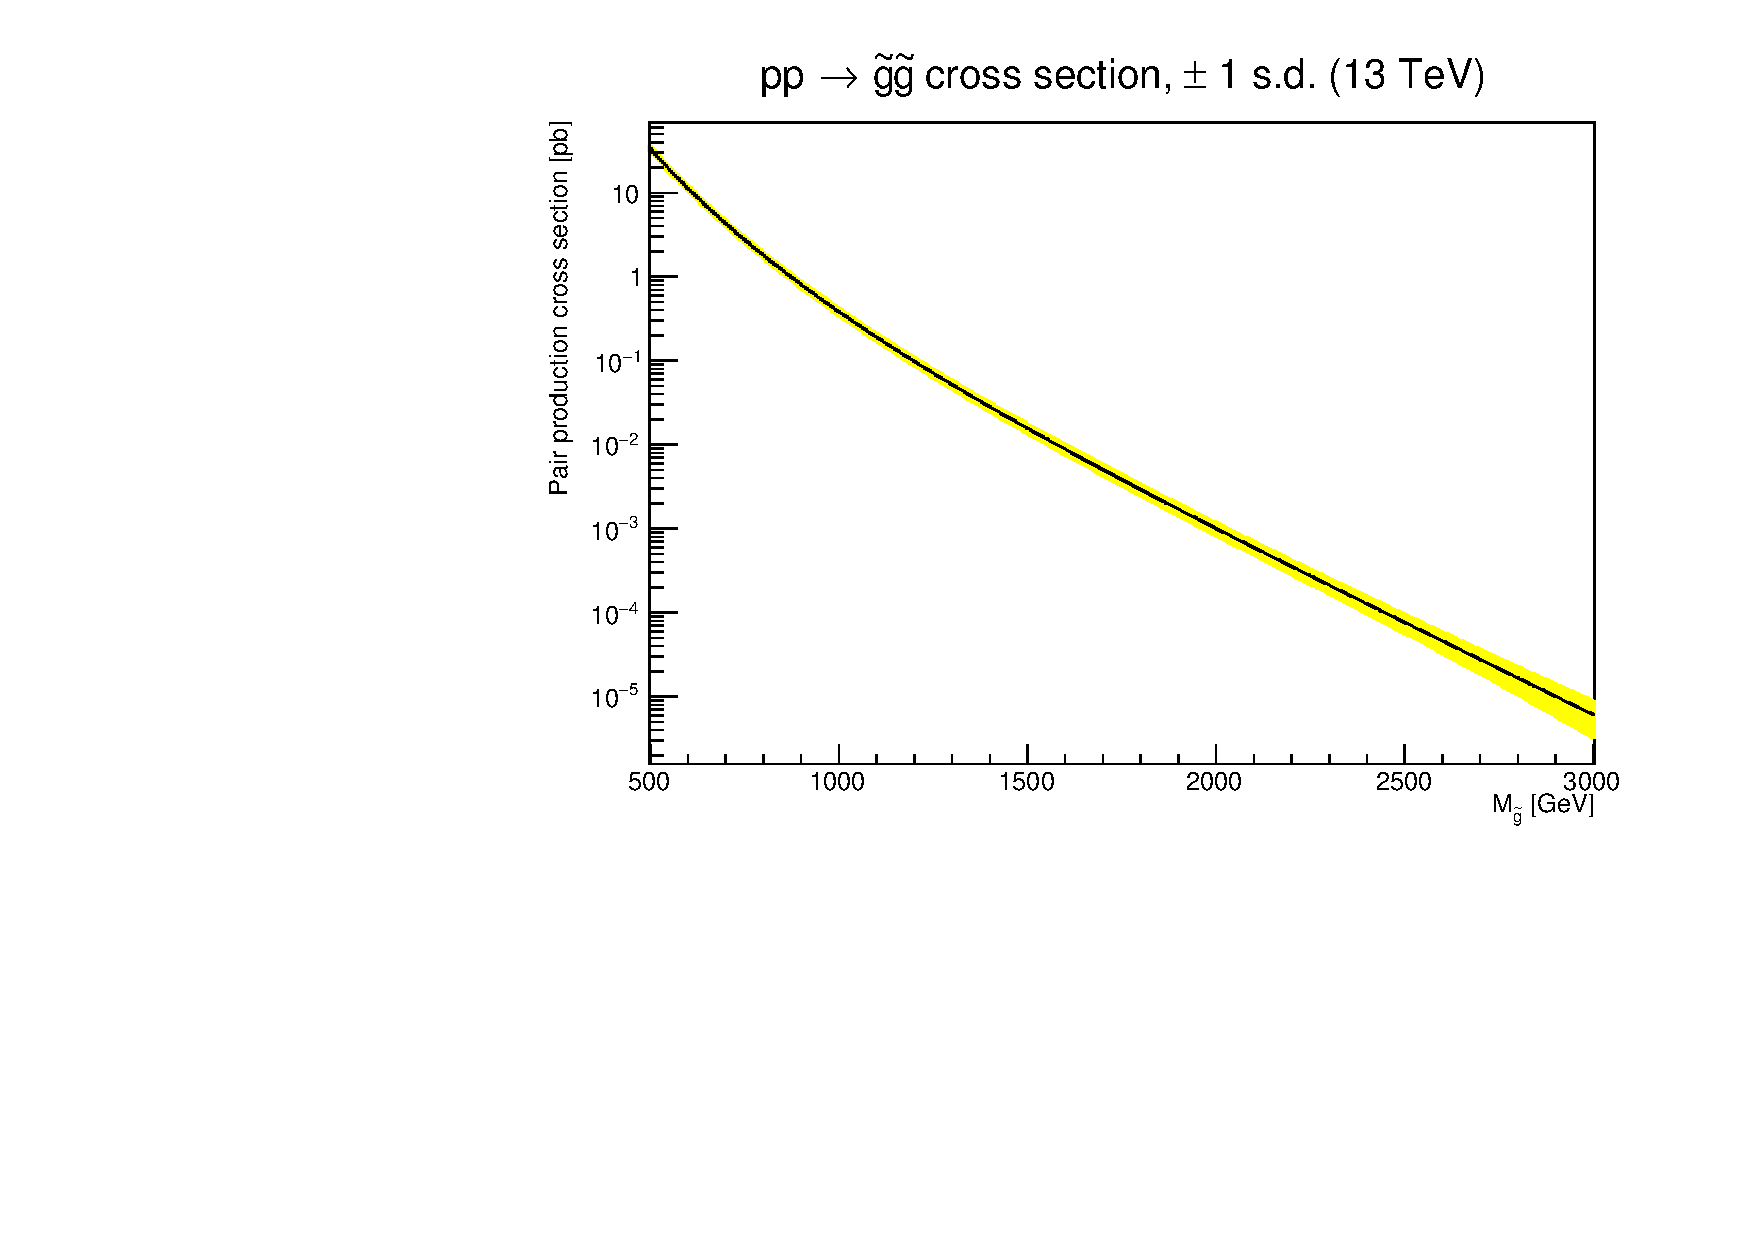
\includegraphics[width=0.85\textwidth]{figures/gluino_xsec.pdf}
    \caption[Theoretical gluino pair production cross section in simplified models.]{In simplified models, it is possible to calculate superpartner production cross sections from theory.
Here, the theoretical gluino pair production cross section in 13 TeV proton-proton collisions is shown in black, with the one standard deviation uncertainty shown as a yellow band.
The cross section drops rapidly with increasing mass.
Based on cross section values used in \cite{MT2_2019}, calculated in \cite{SUSYxsecs}.
Compare Figure 5 (upper) from \cite{SUSYxsecs}, of which this is a simplified reproduction.
}
    \label{fig:SUSYxsec}
  \end{figure}  

\section{Other Models} \label{sec:othermodels}

Introduce leptoquarks and mono-$phi$.

